\documentclass[12pt]{article}

\usepackage[margin=2cm]{geometry}
\usepackage{amsmath}
\usepackage{multicol}
\usepackage{nopageno}
\usepackage{SIunits}
\usepackage{graphicx}
\usepackage{enumerate}
%\usepackage{mathabx}
\usepackage{wasysym}

%%%%%%%%%%%%%%%%%%%%%%%%%%%%%%%%%%%%%%%%%%%%%%%%%%%%%
% For putting links in the document (both to sections and hyperlinks)
\usepackage{hyperref}
\usepackage{url}
\hypersetup{
    colorlinks=true,     % false: boxed links; true: colored links
    linkcolor=red,       % color of internal links
    citecolor=blue,      % color of links to bibliography
    filecolor=blue,      % color of file links
    urlcolor=blue        % color of external links
}
% below, use \url{http://www.nytimes.com} (they will be urlcolor)
%%%%%%%%%%%%%%%%%%%%%%%%%%%%%%%%%%%%%%%%%%%%%%%%%%%%%


%%%%%%%%%%%%%%%%%%%%%%%%%%%%%%%%%%%%%%%%%%%%%%%%%%%%%
% for the events page boxes

% boxed regions
\usepackage{tcolorbox}
\tcbuselibrary{skins,breakable}

% fonts & spacing
\usepackage{lmodern}
\usepackage{microtype}
\usepackage{calc}


% small helper macros (adjust these)
\newcommand{\boxheight}{4.2cm}   % height for each event box
\newcommand{\boxfont}{\scriptsize} % change to \tiny or \footnotesize as desired
\newcommand{\linelen}{0.95\linewidth} % timeline line length

%%%%%%%%%%%%%%%%%%%%%%%%%%%%%%%%%%%%%%%%%%%%%%%%%%%%%
\newcommand{\rmd}{\ensuremath{{\rm d}}}
%\newcommand{\vv}[1]{\ensuremath{\vec{#1}}}
\newcommand{\vv}[1]{\ensuremath{\mathbf{#1}}}
\newcommand{\ee}[1]{\ensuremath{\mathbf{e}_{#1}}}
%%%%%%%%%%%%%%%%%%%%%%%%%%%%%%%%%%%%%%%%%%%%%%%%%%%%%



\begin{document}

\begin{center}
{\Large Contemporary Climate Change: How do we know what we know?}
\end{center}

%\noindent nothing


%%%%%%%%%%%%%%%%%%%%%%%%%%%%%%%%%%%%%%%%%%%%%%%%%%%%
%%%%%%%%%%                                  Questions                                %%%%%%%%%%%%%%%%
%%%%%%%%%%%%%%%%%%%%%%%%%%%%%%%%%%%%%%%%%%%%%%%%%%%%
\begin{enumerate}

\item {\bf Detection of Climate Change} 
	%
	\begin{enumerate}[(a)]
	\item In the reading and in lab this week we discussed the ``global average temperature anomaly'' (GATA). Briefly explain how this quantity is defined and how it is calculated, given measurements of temperature from thermometers at various locations on Earth. 
	\item Pointing to specific places on the graph of GATA\footnote{In the figure it is called the ``global mean temperature difference.''} 1850--present (see figures on next pages), comment on: (i) how the methodological {\em uncertainty} in the estimate of the GATA has changed over time (consider for example the comparison of the values from independent groups; try to give quantitative estimates) and, (ii) why the uncertainty might have changed in this way.
	\item Pointing to specific places on the graph, comment on: (i) the natural variability in the {\em value} of the Earth's temperature (Can you give a quantitative estimate for the value of this variabilty in $\degree$C?), and (ii) which features of the data cannot be explained by ``natural variability.''  
	\item Consider now the longer-term temperature graph ---  including both human thermometer measurements since 1850, and geological  ``temperature proxy'' measurements since 25,000 years ago --- comment again on the ``natural variability''  of Earth's temperature, and specifically how we should interpret the change in GATA since 1970.
	%\item Identify at least three of the groups contributing data to the GATA graph (look up their names/acronyms). 
	% Heat islands?
		
	\end{enumerate}

\item {\bf Attribution of Climate Change} Scientists in the ``working group'' for {\em the physical scientific basis of climate change}\footnote{There are two other working groups in the IPCC: WG2 asseses the vulnerability of socioeconomic and natural systems to the effects of climate change, and WG3  assesses options for mitigating climate change.} within the Intergovernmental Panel on Climate Change (IPCC), have use the terminology ``Detection and attribution'' of climate change\footnote{See a complete definition and explanation of the terminology in the 2007 WG1 report \href{https://archive.ipcc.ch/publications_and_data/ar4/wg1/en/ch9s9-1-2.html}{here}, as well as the \href{https://www.ipcc.ch/site/assets/uploads/2018/02/WG1AR5_Chapter10_FINAL.pdf}{AR5 (2018)} report.}.  Problem (1.) addressed the question of detection: Has the climate changed in a statistical sense, i.e., outside of the bounds of instrumental and methodological uncertainty, and natural variation? (I think your answer to that question is ``yes.'')  Here we consider the {\em attribution} question: To what can we attribute these changes; what is their cause?  This is often stated more specifically as: Can the detected increase in GATA be confidently attributed to human greenhouse gas production?
	%
	\begin{enumerate} 
	\item Consider the information presented in the lecture slides (see ``Class Slides'' on Blackboard, possibly supplemented by Nadir Jeevanjee's original talk).  State and briefly explain 2--3 pieces of evidence that support the argument that our warming climate can indeed be attributed to greenhouse gas (primarily $\text{CO}_2$) production.
	\item Consider the 2008  Geophysical Research Letters paper by Lean et.\ al.\ \footnote{From Lean et.\ al.\ {\em How natural and anthropogenic influences alter global and regional surface temperatures: 1889 to 2006} (\href{https://agupubs.onlinelibrary.wiley.com/doi/full/10.1029/2008GL034864}{Geophys Res Lett 2008})}, whose abstract and first two figures are shown on a later page.  (i) What do they mean by a ``robust multivariate analysis''?  (ii) What is the connection between the data shown in Figure 1 and the overplotted green line on the temperature graph of Figure 2?  (iii) What is the overall conclusion of this analysis?
	\item There is another interesting piece of evidence that allows us to attribute warming to greenhouse gas emissions, which is often called the ``human fingerprint'' of temperature change.  (i) Read the abstract of Santer et al (PNAS 2023) linked on Blackboard and describe what the effect is. (ii) Using Figure 1 of their paper, discuss how they have observed the effect.
	\end{enumerate}

%\item {\bf Temperature and Carbon Dioxide}  
%	%
%	\begin{enumerate}
%	\item Look at CO2 and temperature over past million years. How did they measure this?  What do you notice about the two graphs?
%	\end{enumerate}
%	
	
%\item {\bf Your local climate change}  
%	%
%	\begin{enumerate}
%	\item Using the scripts provided, demonstrate the change in climate in Grand Rapids in three ways: histogram of one month's temperature  (1960 decade vs 2010 decade); monthly average temperatures (1960 decade vs 2010 decade)
%	\end{enumerate}

\end{enumerate}


\newpage
%%%%%%%%%%%%%%%%%%%%%%%%%%%%%%%%%%%%%%%%%%%%%%%%%%%%
%%%%%%%%%%                                  GATA Graph                                %%%%%%%%%%%%%%%%
%%%%%%%%%%%%%%%%%%%%%%%%%%%%%%%%%%%%%%%%%%%%%%%%%%%%

\begin{center}
\includegraphics[width=0.8\textwidth]{images/global-average-temperature_met-office_2025-09_rotated.png}
\end{center}

\newpage
%%%%%%%%%%%%%%%%%%%%%%%%%%%%%%%%%%%%%%%%%%%%%%%%%%%%
%%%%%%%%%%                    25,000y temperature graph                 %%%%%%%%%%%%%%%%
%%%%%%%%%%%%%%%%%%%%%%%%%%%%%%%%%%%%%%%%%%%%%%%%%%%%

\begin{center}
\includegraphics[width=\textwidth]{images/row4_25kya.pdf}
\end{center}

\newpage
%%%%%%%%%%%%%%%%%%%%%%%%%%%%%%%%%%%%%%%%%%%%%%%%%%%%
%%%%%%%%%%                      Lean (GRL 2008) Paper                     %%%%%%%%%%%%%%%%
%%%%%%%%%%%%%%%%%%%%%%%%%%%%%%%%%%%%%%%%%%%%%%%%%%%%

\begin{center}
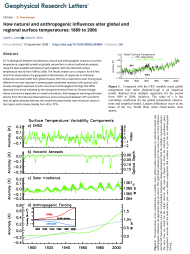
\includegraphics[width=\textwidth]{images/lean2008.pdf}
\end{center}


\vspace{2cm} 
\newpage
%%%%%%%%%%%%%%%%%%%%%%%%%%%%%%%%%%%%%%%%%%%%%%%%%%%%
%%%%%%%%%%                      Santer (PNAS 2023) Paper                     %%%%%%%%%%%%%%%%
%%%%%%%%%%%%%%%%%%%%%%%%%%%%%%%%%%%%%%%%%%%%%%%%%%%%

\begin{center}
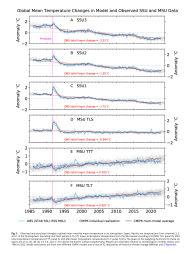
\includegraphics[width=\textwidth]{images/santer2023.pdf}
\end{center}


\vspace{2cm} 

%%%%%%%%%%%%%%%%%%%%%%%%%%%%%%%%%%%%%%%%%%%%%%%%%%%%
%%%%%%%%%%                                  References                                %%%%%%%%%%%%%%%%
%%%%%%%%%%%%%%%%%%%%%%%%%%%%%%%%%%%%%%%%%%%%%%%%%%%%
%\noindent {\bf Data Sources}: 



\end{document}
